\subsubsection{Introduction}
%LET'S GO TEAM!!! ONE LESS SECTION
%We are unstoppppable --> DAB DAB DAB

Due to the non sphericity of the Earth, two deviations exist in terms of perigee and ascendent node. This perturtions are related to the J2 effect descrived before.
Both effects are related to the orbital planes inclination angle, so depending in which inclination they are positionated, the perturbation will be more or less  significant.

\begin{figure}[H] %[b] % h / H / b / t
	\centering
	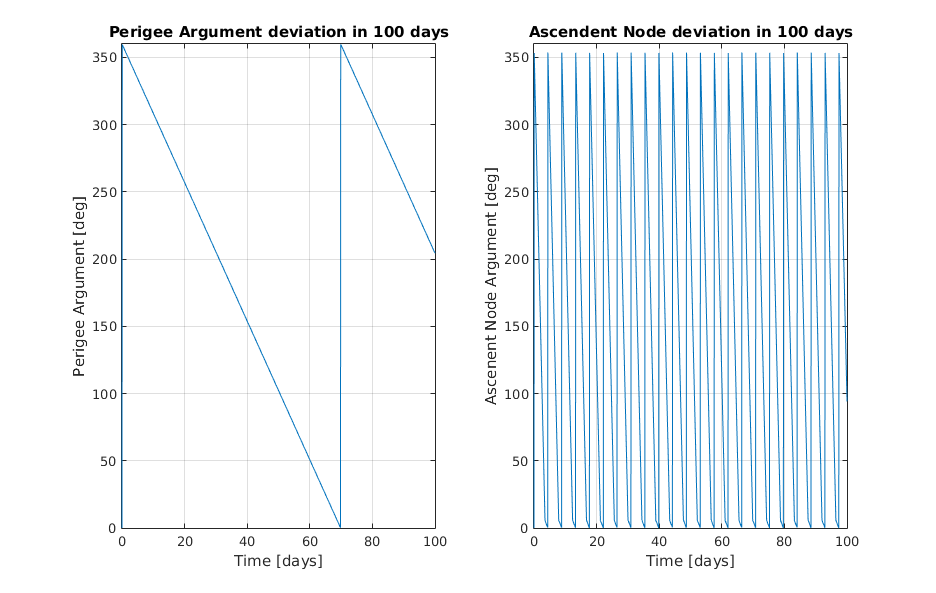
\includegraphics[width=.8\textwidth]{./decay/Inclination.png}\\
	\caption{Ascention node perturbation\\
			On the left: Perigee deviation in terms of time.\\
			On the right: Ascending node deviation in terms of time}
	\label{fig:Inclination} 
\end{figure}

\subsubsection{Perigee Effect}

The Perigee effect is the responsible of the rotation of the orbit regarding the Earth and is found inside the orbital plane itself. Therefore the perigee of an eliptical orbit is not static in an Earth's point but moves around it. 

This effect is noticed when having eliptical orbits. Consequently Astrea constellation will not be affected because the satellites describe almost circular orbits.


\subsubsection{Ascention Node}

In this case the perturbation affects the rotation of the orbital plane. So the plan longitude variates with time. That means, that if we had just one orbital plane it would not cover always the same fraction of Earth.

This effect is noticed when having planes with different inclinitations. That is not Astrea's constellation case since all its planes are positioned in the same inclination angle.


\subsubsection{Conclusion}

As explained, both perturbations do not affect Astrea's constellation so they will not be considered as atctive agents on the orbit decay proces

The Figure~\ref{fig:Inclination} shows the propagation in time of both effects which are periodic due to the constant velocity  of orbits.




